\subsection{Principal fiber bundles}

DEFINITION 1. --- Let G be a topological group and B a topological space. A (right) principal fiber bundle with base B and group G is a B-space (E, p) equipped with a right action of G on E (A, I, p. 50) having the following property:

(FP) For every point \(b\) of \(B\), there exists a neighborhood \(U\) of \(b\) and a U-isomorphism \(f\colon U\times G\to \overline{p}^{1}(U)\) such that for all \(u\in U\) and \(g,g'\in G\), one has \(f(u,gg')=f(u,g)\cdot g'\).

Instead of saying that \((E, p)\) is a principal fiber bundle with base B and group G, one sometimes says that the quadruple \((E, G, B, p)\) is a principal fibration (cf. VAR, R, §6), or by abuse of language that the map \(p: E \to B\) is a principal fibration with base B and group G.

When no doubt is possible as to the base B, the group G, and the action of G on E, we will simply say that \((E, p)\) is a principal fiber bundle.

Let G be a topological group. Let \((E,p)\) be a B-space equipped with a left action of G. If, for the right action of the group \(G^{\circ}\), opposite to the given operation (A, I, p. 50), \((E,p)\) is a principal right fiber bundle with group \(G^{\circ}\), we say that \((E,p)\) is a principal left fiber bundle with group G.

A principal fiber bundle is a locally trivial fiber bundle (I, p. 68, def. 1).

It follows from property (FP) that the group G acts continuously (TG, III, p. 9) and freely on E, and that the orbits of this action are the fibers of the B-space (E, p). The map \(p' \colon \mathrm{E} / \mathrm{G} \to \mathrm{B}\) deduced from \(p\) is continuous and bijective. Again by property (FP), the map \(p\) is open (TG, I, p. 30, prop. 2 and p. 26, prop. 5); consequently, \(p'\) is a homeomorphism (TG, I, p. 32, prop. 3).

Let \((\mathrm{E},p)\) and \((\mathrm{E}^{\prime},p^{\prime})\) be principal fiber bundles with base B and group G. We say that a map \(f: E \to E^{\prime}\) is a morphism of principal fiber bundles (with base B and group G) if f is a B-morphism and one has \(f(x \cdot g) = f(x) \cdot g\) for all \(x \in E\) and every \(g \in G\). Let \((\mathrm{E}^{\prime\prime},p^{\prime\prime})\) be a principal fiber bundle with base B and group G. If \(f: \mathrm{E} \to \mathrm{E}'\) and \(g: \mathrm{E}' \to \mathrm{E}''\) are morphisms of principal fiber bundles, the map \(g \circ f: \mathrm{E} \to \mathrm{E}''\) is a morphism of principal fiber bundles. In accordance with the general definitions (E, IV, p. 11), one may take as morphisms of the principal fiber-bundle structure with base B and group G those defined above. We denote \(\mathcal{C}_{\mathrm{B}}^{\mathrm{G}}(\mathrm{E}; \mathrm{E}')\) the set of morphisms of principal fiber bundles from \((\mathrm{E}, p)\) to \((\mathrm{E}',p')\).

We call the trivial principal fiber bundle with base B and group G the B-space \((B \times G, pr_{1})\) endowed with the right action of G on \(B \times G\) defined by \((b, g) \cdot h = (b, gh)\) .

A principal fiber bundle (E, p) with base B and group G is said to be trivializable if there exists an isomorphism from (E, p) onto the trivial principal fiber bundle \((B \times G,\mathrm{pr}_{1})\); such an isomorphism is called a trivialization of the principal fiber bundle (E, p). Property (FP) expresses that there exists an open covering \((\mathrm{U}_{i})_{i \in \mathrm{I}}\) of B such that, for every \(i \in I\), the \(\mathrm{U}_{i}\)-space \((\overline{p}^{1}(\mathrm{U}_{i}), p \mid \mathrm{U}_{i})\), endowed with the right action of G induced by that of G on E, is a trivializable principal fiber bundle.

Examples. --- 1) Let (E, p) be a principal fiber bundle with base B and group G, and let A be a subspace of B. The subspace \(E_{A} = \overline{p}^{1}(A)\) of E is stable under the action of G, and the map \(p_{A}: E_{A} \to A\) makes it a principal fiber bundle with base A and group G. One says that \((E_{A}, p_{A})\) is the principal fiber bundle induced by (E, p) over A.

\begin{enumerate}
\def\labelenumi{\arabic{enumi})}
\setcounter{enumi}{1}
\tightlist
\item
  Let (E, p) be a principal fiber bundle with base B and group G; let \((\mathrm{E}^{\prime}, p^{\prime})\) be a principal fiber bundle with base \(B^{\prime}\) and group \(G^{\prime}\). One defines a right action of the group \(G \times G^{\prime}\) on the space \(E \times E^{\prime}\) by setting \((x, x^{\prime}) \cdot (g, g^{\prime}) = (x \cdot g, x^{\prime} \cdot g^{\prime})\) for \(x \in E\), \(x^{\prime} \in E^{\prime}\), \(g \in G\) and \(g^{\prime} \in G^{\prime}\); this action is continuous. Let U be an open subset of B and \(f: U \times G \to \overline{p}^{1}(U)\) a trivialization of the U-space \((\overline{p}^{1}(U), p_{\mathrm{U}})\); let \(U^{\prime}\) be an open subset of \(B^{\prime}\) and \(f^{\prime}: U^{\prime} \times G^{\prime} \to \overline{p'}^{1}(U^{\prime})\) a trivialization of the \(U^{\prime}\)-space \((\overline{p'}^{1}(U^{\prime}), p_{\mathrm{U}}^{\prime})\). The map \(((b, b^{\prime}), (g, g^{\prime})) \mapsto (f(b, g), f'(b', g'))\) is a \((\mathrm{U} \times \mathrm{U}^{\prime})\)-isomorphism \(f''\) of \((\mathrm{U} \times \mathrm{U}^{\prime}) \times (\mathrm{G} \times \mathrm{G}^{\prime})\) onto \(\overline{p}^{1}(U) \times \overline{p'}^{1}(U^{\prime})\) and one has
\end{enumerate}

\[
f ^ {\prime \prime} ((b, b ^ {\prime}), (g h, g ^ {\prime} h ^ {\prime})) = (f (b, g h), f ^ {\prime} (b ^ {\prime}, g ^ {\prime} h ^ {\prime})) = f ^ {\prime \prime} ((b, b ^ {\prime}), (g, g ^ {\prime})) \cdot (h, h ^ {\prime}).
\]

It follows that the \((\mathrm{B} \times \mathrm{B}')\)-space \(E \times E'\), endowed with the action of \(G \times G'\) defined above, is a principal fiber bundle, called the product of the principal fiber bundles E and E'.

\begin{enumerate}
\def\labelenumi{\arabic{enumi})}
\setcounter{enumi}{2}
\item
  In particular, when \(B = B'\) , the B-space \(E \times_{B} E'\) is identified with the principal fiber bundle with group \(G \times G'\) induced by \(E \times E'\) over the diagonal \(\Delta_{B}\) of \(B \times B\) . Endowed with this principal fiber bundle structure, the B-space \(E \times_{B} E'\) is called the fibered product of the principal fiber bundles E and \(E'\) .
\item
  Let E be a principal fiber bundle with base B and group G, and let F be a topological space. The \((B \times F)\) -space \(E \times F\) endowed with the action \((x, y) \cdot g = (x \cdot g, y)\) , for \(x \in E\) , \(y \in F\) and \(g \in G\) , is a principal fiber bundle with group G. This is the particular case of Example 2, where \(p'\) is the identity map of F and \(G'\) is a group reduced to the identity element.
\item
  Let B be a topological space and (E, p) a principal fiber bundle with base B and group G. Let B' be a topological space and \(f: B' \to B\) a continuous map. The group G acts on the right on the fibered product \(B' \times_{B} E\) by the law \((b', x) \cdot g = (b', x \cdot g)\) , for \(b' \in B'\) , \(x \in E\) and \(g \in G\) . This action is continuous and free; the orbits are the fibers of the map \(pr_{1}: B' \times_{B} E \to B'\) . It follows from Examples 1 and 4 above and from Remark 2 of I, p. 16 that the \(B'\) -space \(B' \times_{B} E\) is a principal fiber bundle with group G. It is called the principal fiber bundle deduced from (E, p) by the base change f, or also the inverse image of (E, p) under f.
\end{enumerate}

PROPOSITION 1. --- Every morphism of principal fiber bundles is an isomorphism.

Let \(f \colon \mathrm{B} \times \mathrm{G} \to \mathrm{B} \times \mathrm{G}\) be a morphism of the trivial principal fiber bundle \((\mathrm{B} \times \mathrm{G},\mathrm{pr}_1)\) into itself and let \(\varphi \colon \mathrm{B} \times \mathrm{G} \to \mathrm{G}\) be the continuous map \(\mathrm{pr}_2 \circ f\), such that \(f(b, g) = (b, \varphi(b, g))\). For all \(b \in \mathrm{B}\) and all \(g, h \in \mathrm{G}\), we have \(\varphi(b, gh) = \varphi(b, g) \cdot h\), whence \(\varphi(b, g) = \varphi(b, e) \cdot g\), where \(e\) denotes the identity element of \(\mathrm{G}\). The morphism \(f\) is therefore an isomorphism whose inverse morphism \(f^{-1}\) is defined by \(f^{-1}(b, g) = (b, \varphi(b, e)^{-1}g)\) for \((b, g) \in \mathrm{B} \times \mathrm{G}\).

Now let E and \(E'\) be principal fiber bundles and let \(f: E \to E'\) be a morphism of principal fiber bundles. Given property (FP), for every point \(b \in B\) there exists an open neighborhood U of b such that the principal bundles \(E_{U}\) and \(E'_{U}\) are trivializable.

By passing to subspaces, \(f\) induces a morphism \(f_{\mathrm{U}}: \mathrm{E}_{\mathrm{U}} \to \mathrm{E}_{\mathrm{U}}'\) of principal fiber bundles; according to the preceding, this morphism \(f_{\mathrm{U}}\) is an isomorphism. In particular, \(f_{b}: \mathrm{E}_{b} \to \mathrm{E}_{b}'\) is a bijection. There then exists a unique map \(g: \mathrm{E}' \to \mathrm{E}\) that induces the bijection \(f_{b}^{-1}\) by passing to subspaces. According to Proposition 4 of I, p. 19, the map \(g\) is continuous; therefore \(f\) is an isomorphism of principal fiber bundles.

COROLLARY. --- Let G be a topological group, \((E, p)\) and \((E', p')\) be principal fiber bundles with group G and bases B and B' respectively. Let \(f: B' \to B\) and \(f': E' \to E\) be continuous maps such that \(p \circ f' = f \circ p'\) and such that, for every \(x' \in E'\) and every \(g \in G\), \(f'(x' \cdot g) = f'(x') \cdot g\). Then the square

\pandocbounded{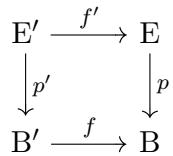
\includegraphics[keepaspectratio]{images/part001_eb35a58e.jpg}}

is a Cartesian square.

Indeed, the map \(h: E' \to B' \times_{B} E\) defined by \(h(x') = (p'(x'), f'(x'))\) is a \(B'\)-morphism of principal fiber bundles, hence an isomorphism; moreover, we have \(pr_{2} \circ h = f'\), whence the result (I, p. 8, prop. 2).

Under the hypotheses of the preceding corollary, one sometimes says that \(f'\) is an f-morphism of principal fiber bundles.

PROPOSITION 2. --- Let (E, p) be a principal fiber bundle with base B and group G, and let \(\varepsilon\) be the section \(b \mapsto (b, e)\) of the trivial principal fiber bundle (B \(\times\) G, \(\mathrm{pr}_{1}\)), where \(e\) denotes the identity element of G. The map \(h \mapsto h \circ \varepsilon\) is a bijection from \(\mathcal{C}_{\mathrm{B}}^{\mathrm{G}}(\mathrm{B} \times \mathrm{G}; \mathrm{E})\) onto the set \(\mathcal{S}(\mathrm{B}; \mathrm{E})\) of continuous sections of \(p\). The inverse bijection associates to a continuous section \(s\) of \(p\) the B-morphism \((b, g) \mapsto s(b) \cdot g\).

COROLLARY. --- A principal fiber bundle is trivializable if and only if it admits a continuous section.

PROPOSITION 3. --- Let E and B be topological spaces, \(p\colon\mathrm{E}\to\mathrm{B}\) a continuous map and G a topological group acting on the right on E. The following conditions are equivalent:

\begin{enumerate}
\def\labelenumi{(\roman{enumi})}
\item
  Endowed with the map p, E is a principal fiber bundle with base B and group G;
\item
  For every \(x \in E\) and every \(g \in G\) , we have \(p(x \cdot g) = p(x)\) , the map \(\theta: (x, g) \mapsto (x, x \cdot g)\) is a homeomorphism of \(E \times G\) onto \(E \times_{B} E\) and every point of B has a neighborhood on which there exists a continuous section of the map p.
\end{enumerate}

(i)⇒(ii): Suppose that (E, p) is a principal fiber bundle. The group G acts continuously and freely on E with the fibers of p as orbits. Consequently, the map \(\theta\) is bijective and continuous. More precisely, if one equips \(E \times_{B} E\) with the action of G defined by \((x, y) \cdot g = (x, y \cdot g)\), the map \(\theta\) is an E-morphism of the trivial principal fiber bundle \(E \times G\) into the principal fiber bundle \((E \times_{B} E \to E, \mathrm{pr}_{1})\) (Example 5), hence an isomorphism (Proposition 1). The other assertions of (ii) follow immediately from the definition.

(ii)⇒(i): Set \(\varphi = pr_{2} \circ \theta^{-1}\) , so that, for every \((x, y) \in E \times_{B} E\) , we have

\[
\theta^ {- 1} (x, y) = (x, \varphi (x, y)).\tag{1}
\]

The map \(\varphi\colon\mathrm{E}\times_{\mathrm{B}}\mathrm{E}\to\mathrm{G}\) is continuous and, for \((x,y)\in\mathrm{E}\times_{\mathrm{B}}\mathrm{E}\), the element \(\varphi(x,y)\) is the unique element \(g\) of G such that \(y=x\cdot g\). Let \(b\) be a point of B; let U be a neighborhood of \(b\) and let \(s\) be a continuous section of \(p\) above U. For \((u,g)\in\mathrm{U}\times\mathrm{G}\), set \(f(u,g)=s(u)\cdot g\); the map \(f\) is a U-morphism from \(U \times G\) to \(\overline{p}^{-1}(\mathrm{U})\). For \(y\in\overline{p}^{-1}(\mathrm{U})\), set \(f'(y)=(p(y),\varphi(s(p(y)),y))\). The map \(f'\) is a U-morphism from \(\overline{p}^{-1}(\mathrm{U})\) to U \(\times\) G. We have

\[
(f \circ f ^ {\prime}) (y) = s (p (y)) \cdot \varphi (s (p (y)), y) = y.
\]

On the other hand, for \((u,g)\in \mathrm{U}\times \mathrm{G}\) , we have

\[
(f ^ {\prime} \circ f) (u, g) = f ^ {\prime} (s (u) \cdot g) = (u, \varphi (s (u), s (u) \cdot g)) = (u, g).
\]

Therefore, f is a U-isomorphism. It follows that \((E,p)\) is a principal fiber bundle with base B and group G.

Remark 1. --- Let (E, p) be a principal fiber bundle with base B and group G. With the notation of Proposition 3, the map \(\theta^{-1}\colon E \times_{B} E \to E \times G\) is a trivialization of the principal fiber bundle \(\mathrm{pr}_{1}\colon E \times_{B} E \to E\). One says that \(\theta^{-1}\) is the canonical trivialization of this principal fiber bundle.

COROLLARY 1. --- Let G be a topological group acting continuously on the right on a topological space E. The following conditions are equivalent:

\begin{enumerate}
\def\labelenumi{(\roman{enumi})}
\item
  The orbit space E/G is Hausdorff, and the space E, equipped with the canonical map \(p: E \rightarrow E/G\), is a principal fiber bundle with group G;
\item
  The group G acts properly (TG, III, p. 27) and freely on E, and every point of E/G has a neighborhood on which there exists a continuous section of the map p.
\end{enumerate}

Set \(B=E/G\). Under each of the hypotheses (i) and (ii), the group G acts continuously and freely on E, so that the map \(\theta\colon(x,g)\mapsto(x,x\cdot g)\) is a continuous bijection from \(E\times G\) onto \(E\times_{B}E\). Let us place ourselves under this hypothesis and denote by \(\varphi\colon E\times_{B}E\to G\) the map \(pr_{2}\circ\theta^{-1}\). Taking formula (1) into account, for \(\theta\) to be a homeomorphism, it is necessary and sufficient that the map \(\varphi\) be continuous. On the other hand, since the equivalence relation defined by G is open (TG, III, p. 10, lemma 2), for the space E/G to be Hausdorff, it is necessary and sufficient that the graph \(E\times_{B}E\) of this equivalence relation be closed in \(E\times E\). For G to act properly on E, it is necessary and sufficient that \(E\times_{B}E\) be closed in \(E\times E\) and that the map \(\varphi\) be continuous. The equivalence of conditions (i) and (ii) then follows from Proposition 3.

COROLLARY 2. --- Let G be a topological group, let H be a subgroup of G, and let p: G → G/H be the canonical map. If the map p admits a continuous section over a nonempty open set of G/H, then p makes G a principal fiber bundle with base G/H and group H.

By left translations, every point of G/H has a neighborhood over which the map p has a continuous section. On the other hand, for \((g,g')\) belonging to \(G\times G\), set \(\varphi(g,g')=g^{-1}g'\). If \(p(g)=p(g')\), \(\varphi(g,g')\) belongs to H. The map \((g,g')\mapsto(g,\varphi(g,g'))\) from \(G\times_{G/H}G\) to \(G\times H\) is continuous and is the inverse of the continuous map \(\theta: G\times H\to G\times_{G/H}G\) defined by \(\theta(g,h)=(g,gh)\), whence the corollary.

Remark 2. --- This situation arises in particular when G is a real Lie group, of finite dimension, countable at infinity, acting transitively and analytically on an analytic manifold X. If one takes for H the stabilizer of a point of X, the map p is a submersion of G onto the homogeneous Lie space G/H, isomorphic to X (LIE, III, p. 109, corollary). It therefore admits local sections (VAR, p. 50).
% semantic-fragments: legacy-input-seam
\relax{}
